\documentclass[11pt,a4paper]{article}

\usepackage[utf8]{inputenc}
\usepackage[T1]{fontenc}
\usepackage[spanish, es-nodecimaldot]{babel}
\addto\captionsspanish{\renewcommand{\tablename}{Tabla}}
\usepackage{geometry}
\geometry{margin=2.5cm}
\usepackage{booktabs}
\usepackage{array}
\usepackage{multirow}
\usepackage{hyperref}
\hypersetup{colorlinks=true, linkcolor=black, urlcolor=blue}
\usepackage{parskip}
\usepackage{listings}
\usepackage{xcolor}
\usepackage{enumitem}
\usepackage{graphicx}
\usepackage{url}
\graphicspath{{diagrams/}}
\usepackage{float}
\usepackage{caption}
\usepackage{rotating}
\usepackage{pdflscape}
\usepackage{colortbl}
\usepackage{amssymb}
\usepackage{inconsolata}

\usepackage{color}

% ---- Colores (mismos que en rediseno-potenciales) ----------------
\definecolor{pblue}{rgb}{0.13,0.13,1}
\definecolor{pgreen}{rgb}{0,0.5,0}
\definecolor{pred}{rgb}{0.9,0,0}
\definecolor{pgrey}{rgb}{0.46,0.45,0.48}

\definecolor{lightgray}{gray}{0.92}
\definecolor{codered}{RGB}{180,30,30}
\definecolor{codegreen}{RGB}{0,120,0}
\definecolor{codegray}{RGB}{100,100,100}
\definecolor{warnorange}{RGB}{200,100,0}

% ---- lstset (identico al de rediseno-potenciales) ----------------
\lstset{
  language=Java,
  basicstyle=\ttfamily\footnotesize,
  keywordstyle=\color{pblue},
  commentstyle=\color{codegray}\itshape,
  stringstyle=\color{pred},
  showstringspaces=false,
  showspaces=false,
  showtabs=false,
  breaklines=true,
  breakatwhitespace=false,
  postbreak=\mbox{\textcolor{codegray}{$\hookrightarrow$}\space},
  frame=single,
  framesep=4pt,
  xleftmargin=6pt,
  xrightmargin=6pt,
  aboveskip=6pt,
  belowskip=6pt,
  numbers=left,
  numberstyle=\tiny\color{codegray},
  numbersep=5pt,
  captionpos=b,
  moredelim=[il][\textcolor{pgrey}]{$$},
  moredelim=[is][\textcolor{pgrey}]{\%\%}{\%\%}
}
\renewcommand{\lstlistingname}{Listado}

% ---- Comandos de texto ------------------------------------------
\newcommand{\code}[1]{\texttt{#1}}
\setlength{\emergencystretch}{3em}
\newcommand{\bad}[1]{\textcolor{codered}{\textbf{#1}}}
\newcommand{\good}[1]{\textcolor{codegreen}{\textbf{#1}}}
\newcommand{\warn}[1]{\textcolor{warnorange}{\textbf{#1}}}

\title{Redise\~no de la clase \code{ProbNet}\\
       \large Motivaciones, decisiones y resultado\\[4pt]
       \normalsize \code{org.openmarkov.core} --- paquete \code{model.network}}
\author{Manuel Arias}
\date{Abril de 2026}

\begin{document}

\maketitle
\tableofcontents
\newpage

% ===================================================================
\section*{Resumen}

\code{ProbNet} es la clase más crítica de OpenMarkov: \textbf{490~ficheros}
la referencian en todo el proyecto.  Con \textbf{1440~líneas} y más de
\textbf{80~métodos públicos} distribuidos en seis áreas de responsabilidad
distintas, la clase había acumulado más trabajo del que le correspondía.

Este documento describe \emph{qué} se cambió, \emph{por qué} se tomó
cada decisión y \emph{cuál es el resultado} en términos de arquitectura
y métricas de código.  El documento de análisis previo
(\emph{Análisis de la clase \code{ProbNet}}) recoge el diagnóstico
detallado; aquí se parte de él y se documenta la ejecución.

% ===================================================================
\section{Fundamentos de ingeniería del software}
\label{sec:fundamentos}

Antes de explicar los cambios concretos conviene definir los conceptos de
ingeniería del software que se aplican a lo largo del documento.  Esta
sección es especialmente útil para lectores con poca experiencia en diseño
orientado a objetos, ya que los términos técnicos se usan con precisión en
el resto del texto.

% -------------------------------------------------------------------
\subsection{Principios de diseño orientado a objetos}
\label{sec:fund-principios}

Los \emph{principios de diseño} son reglas generales que, cuando se
aplican con criterio, producen código más fácil de entender, modificar
y probar.  No son recetas infalibles, sino guías para tomar decisiones
de diseño razonadas.

% - - - - - - - - - - - - - - - - - - - - - - - - - - - - - - - - -
\label{sec:fund-srp}
\paragraph{Principio de Responsabilidad Única (SRP).}

El \emph{Single Responsibility Principle} establece que \textbf{una
clase debe tener una sola razón para cambiar}~\cite{martin2003}.  Si
un módulo hace demasiadas cosas a la vez, cualquier cambio en una de
ellas obliga a revisar y probar todas las demás.
% - - - - - - - - - - - - - - - - - - - - - - - - - - - - - - - - -
\label{sec:fund-dry}
\paragraph{Principio DRY (\emph{Don't Repeat Yourself}).}

El principio DRY establece que \textbf{cada pieza de conocimiento debe
tener una única representación en el sistema}~\cite{hunt1999}.  Cuando
la misma lógica aparece en dos lugares, una corrección o un cambio de
comportamiento debe aplicarse en ambos; si se olvida uno, el código queda
inconsistente.

El ejemplo más directo en \code{ProbNet} era que el método
\code{checkProbNet()} recorría la lista de restricciones con la misma
lógica que \code{getUnsatisfiedConstraints()}, sin reutilizar ese último.

% - - - - - - - - - - - - - - - - - - - - - - - - - - - - - - - - -
\label{sec:fund-dip}
\paragraph{Principio de Inversión de Dependencias (DIP).}

El \emph{Dependency Inversion Principle} establece que \textbf{los
módulos de alto nivel no deben depender de los módulos de bajo
nivel}~\cite{martin2003}.  En diseño orientado a objetos, esto se
concreta en: el modelo de dominio (lo más importante en una aplicación)
no debería conocer los detalles de los sistemas que lo rodean, como la
entrada/salida de ficheros.

Si el modelo sabe cómo leer y escribir ficheros, un cambio en el formato
de archivo puede obligar a modificar el modelo de dominio, que es la parte
más delicada del sistema.

% - - - - - - - - - - - - - - - - - - - - - - - - - - - - - - - - -
\label{sec:fund-composition}
\paragraph{Composición frente a herencia.}

En programación orientada a objetos existen dos formas de reutilizar
comportamiento: la \emph{herencia} (``clase B es un tipo de clase A'')
y la \emph{composición} (``clase B \emph{tiene} un objeto de tipo A'').

La herencia crea un acoplamiento muy fuerte: la subclase hereda
\emph{todo} lo de la clase padre, incluyendo lo que no necesita, y
cualquier cambio en el padre puede romper la subclase.  La composición
es más flexible: el objeto contenido puede cambiarse o sustituirse sin
tocar la clase contenedora.

Un principio clásico de diseño recomienda \textbf{preferir la composición
frente a la herencia} siempre que la relación entre clases no sea
genuinamente ``es un tipo de''~\cite{gamma1995}.

% - - - - - - - - - - - - - - - - - - - - - - - - - - - - - - - - -
\label{sec:fund-isp}
\paragraph{Principio de Segregación de Interfaces (ISP).}

El \emph{Interface Segregation Principle} establece que \textbf{una
clase no debe ser obligada a depender de métodos que no utiliza}.
Es preferible tener varias interfaces pequeñas y específicas que una
sola interfaz grande: así, cada consumidor declara exactamente las
capacidades que necesita, sin verse arrastrado por métodos que nunca
va a llamar.

En la práctica, esto significa que un algoritmo de inferencia que
solo necesita consultar el grafo de la red no debería necesitar importar
toda la clase \code{ProbNet} con sus 80~métodos; debería poder trabajar
con una interfaz más pequeña que defina solo las operaciones de consulta.

% -------------------------------------------------------------------
\subsection{Antipatrones detectados}
\label{sec:fund-antipatrones}

Un \emph{antipatrón} es un patrón recurrente de diseño que, en
apariencia razonable, genera en la práctica problemas de mantenimiento
o fragilidad.  Reconocer los antipatrones en el código propio es el
primer paso para corregirlos.

% - - - - - - - - - - - - - - - - - - - - - - - - - - - - - - - - -
\label{sec:fund-god-class}
\paragraph{God Class (Clase Dios).}

\textbf{Descripción:} una clase que acumula demasiadas responsabilidades:
lo sabe todo y lo hace todo.  En lugar de delegar en otras clases,
concentra lógica de distintos dominios en una sola unidad.

\textbf{Por qué es dañina:} viola directamente el SRP.  Cualquier cambio
requiere entender la clase entera, porque los distintos dominios están
entrelazados.  Las pruebas unitarias son difíciles de escribir por el
elevado número de combinaciones posibles de estado.  La God Class se
convierte en el cuello de botella del desarrollo: todo pasa por ella.

\textbf{Solución habitual:} identificar las distintas responsabilidades
y extraer cada una a su propia clase.  Esto es exactamente lo que la
técnica \emph{Extract Class} persigue.

% - - - - - - - - - - - - - - - - - - - - - - - - - - - - - - - - -
\label{sec:fund-inh-misuse}
\paragraph{Herencia inapropiada.}

\textbf{Descripción:} usar herencia para reutilizar la implementación
de otra clase, aunque la relación ``es un tipo de'' no sea semánticamente
correcta.  El resultado es que la subclase hereda métodos y campos que
no le corresponden y queda atada a todos los cambios del padre.

\textbf{Por qué es dañina:} produce acoplamiento innecesario entre clases
que conceptualmente son independientes.  Además, dificulta el uso de
interfaces: si una clase hereda de una clase concreta, el código cliente
no puede desacoplarse fácilmente de la implementación.

\textbf{Solución habitual:} sustituir la herencia por composición y
declarar las capacidades de la clase mediante interfaces.

% -------------------------------------------------------------------
\subsection{Patrones de diseño aplicados}
\label{sec:fund-patrones}

Un \emph{patrón de diseño} es una solución reutilizable a un problema
frecuente de diseño orientado a objetos~\cite{gamma1995}.  A diferencia
de los antipatrones, los patrones de diseño son soluciones contrastadas.

% - - - - - - - - - - - - - - - - - - - - - - - - - - - - - - - - -
\label{sec:fund-extract-class}
\paragraph{Extract Class (Extraer Clase).}

\textbf{Descripción:} cuando una clase tiene demasiadas
responsabilidades, se identifica un grupo cohesivo de métodos y campos
y se mueve a una nueva clase.  La clase original delega en la nueva
mediante llamadas explícitas.

\textbf{Aplicación en este documento:} se aplica en cinco ocasiones para
reducir \code{ProbNet}: se extraen la clasificación de la red
(\code{ProbNetClassifier}), la gestión de agentes
(\code{ProbNetAgentManager}), las consultas complejas de potenciales
(\code{ProbNetPotentialQueries}), la lógica de copia
(\code{ProbNetCopier}) y los metadatos descriptivos
(\code{NetworkMetadata}).

% - - - - - - - - - - - - - - - - - - - - - - - - - - - - - - - - -
\label{sec:fund-value-object}
\paragraph{Value Object (Objeto Valor).}

\textbf{Descripción:} un objeto que agrupa datos relacionados sin
identidad propia: lo que importa es su contenido, no su dirección en
memoria.  Típicamente es mutable (porque sus datos pueden cambiar) pero
no tiene lógica de negocio compleja.

\textbf{Aplicación en este documento:} \code{NetworkMetadata} agrupa
los metadatos de la red (nombre, comentario, estados por defecto,
criterios, etc.) en un único objeto que \code{ProbNet} posee.  Al
separar los datos de configuración del modelo de dominio en sí, queda
claro qué es infraestructura descriptiva y qué es comportamiento.

% - - - - - - - - - - - - - - - - - - - - - - - - - - - - - - - - -
\label{sec:fund-interface-seg}
\paragraph{Interfaces como contrato mínimo.}

\textbf{Descripción:} en lugar de hacer que todo el código cliente
dependa de una clase concreta grande, se definen interfaces que
describen solo las capacidades que cada cliente necesita.  El cliente
declara su dependencia sobre la interfaz; la clase concreta implementa
todas las interfaces que corresponda.

\textbf{Aplicación en este documento:} se introducen las interfaces
\code{GraphNetwork} y \code{PotentialNetwork} que permiten a los
algoritmos de inferencia declarar exactamente qué vista de la red
necesitan, desacoplándose del tipo concreto \code{ProbNet}.

% ===================================================================
\section{Situación de partida}
\label{sec:antes}

\subsection{La clase en cifras}

\code{ProbNet} era la clase más grande y más referenciada del proyecto.
La Figura~\ref{fig:before} muestra un diagrama UML que agrupa sus
métodos por responsabilidad y señala los problemas detectados.

\begin{figure}[H]
  \centering
  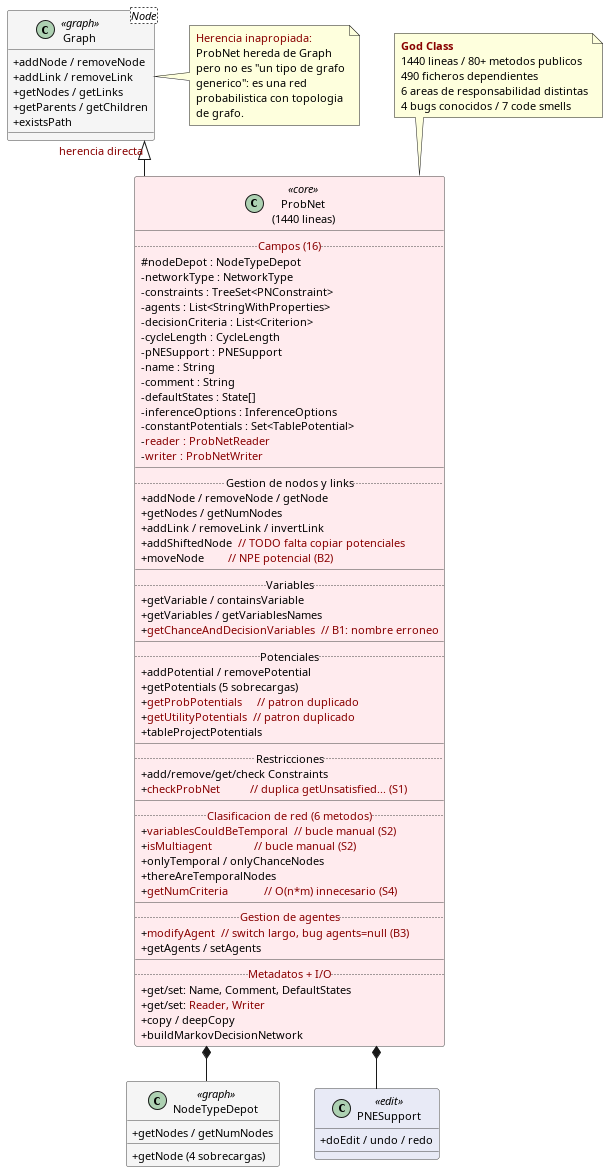
\includegraphics[width=0.8\textwidth]{before.png}
  \caption{Diagrama UML de \code{ProbNet} antes del rediseño (1440~líneas).
           En \textcolor{codered}{\textbf{rojo}} se señalan los problemas
           principales.}
  \label{fig:before}
\end{figure}

\noindent Las cifras más llamativas eran:

\begin{center}
\begin{tabular}{lr}
\toprule
\textbf{Métrica}               & \textbf{Valor} \\
\midrule
Líneas de código                & 1\,440 \\
Métodos públicos                & 80+ \\
Campos                          & 16 \\
Ficheros dependientes           & 490 \\
Áreas de responsabilidad        & 6 \\
Bugs conocidos                  & 4 \\
Code smells documentados        & 7 \\
Cobertura de tests (métodos)    & 37\% \\
\bottomrule
\end{tabular}
\end{center}

Las seis áreas de responsabilidad eran: gestión de nodos/links/variables,
gestión de potenciales, restricciones de red, clasificación de la red,
gestión de agentes y metadatos + I/O.  Cada una de estas áreas responde
a motivos de cambio distintos, lo que convierte a \code{ProbNet} en un
ejemplo claro de God Class (§\ref{sec:fund-god-class}).

\subsection{Herencia directa de \texttt{Graph\textless{}Node\textgreater{}}}

\code{ProbNet} extendía \code{Graph<Node>}, la clase genérica de grafo de
la librería interna.  Esta relación de herencia era inapropiada
(§\ref{sec:fund-inh-misuse}): una red probabilística \emph{usa} un grafo
para representar su topología, pero no \emph{es} un grafo genérico.

La consecuencia práctica era que cualquier código que quisiera
desacoplarse de los detalles de \code{ProbNet} no podía, porque no
existía ninguna interfaz intermedia.  Un algoritmo de inferencia
necesitaba importar la clase concreta aunque solo usara operaciones de
consulta del grafo.

\subsection{Campos \texttt{reader} y \texttt{writer} en el modelo de dominio}

\code{ProbNet} almacenaba referencias a \code{ProbNetReader} y
\code{ProbNetWriter}, los objetos responsables de la lectura y escritura
de ficheros.  Esto era una violación directa del DIP
(§\ref{sec:fund-dip}): el modelo de dominio conocía los detalles del
sistema de I/O.

El motivo por el que estos campos existían era funcional: la GUI necesitaba
saber con qué lector/escritor se había abierto la red para usar el mismo
formato al guardar.  Sin embargo, esa información pertenece al controlador
de ficheros, no al modelo.  El acoplamiento no era necesario, y los campos
permanecen en \code{ProbNet} de momento por compatibilidad con la GUI,
pero ya están aislados dentro de \code{NetworkMetadata}.

\subsection{Bugs conocidos}
\label{sec:bugs}

El análisis previo (véase \emph{Análisis de la clase \code{ProbNet}})
identificó cuatro bugs:

\begin{center}
\begin{tabular}{clp{9cm}}
\toprule
\textbf{Bug} & \textbf{Método} & \textbf{Descripción} \\
\midrule
B1 & \code{getChanceAndDecisionVariables()} &
     El nombre indicaba que devolvía variables CHANCE y DECISION, pero el
     \code{switch} incluía también \code{SV\_PRODUCT} y \code{SV\_SUM}.
     Nombre engañoso o comportamiento incorrecto. \\
B2 & \code{moveNode()} &
     \code{getNode(name)} puede devolver \code{null} si el nombre no
     existe; no había comprobación de nulidad antes de usarlo. \\
B3 & \code{modifyAgent(REMOVE)} &
     Al eliminar el último agente asignaba \code{agents = null}.
     Cualquier llamada posterior a \code{getAgents()} causaba un
     \code{NullPointerException}. \\
B4 & \code{addShiftedNode()} &
     Copiaba el tipo, coordenadas y propiedades del nodo, pero no sus
     potenciales. El propio código tenía un comentario \code{// TODO}
     reconociendo la omisión. \\
\bottomrule
\end{tabular}
\end{center}

\subsection{Code smells}
\label{sec:smells}

Los siete code smells detectados cubrían: duplicación de lógica entre
\code{checkProbNet()} y \code{getUnsatisfiedConstraints()} (violación DRY);
bucles manuales donde existía un método más expresivo; duplicación del
patrón de iteración en \code{getProbPotentials()} y
\code{getUtilityPotentials()}; complejidad $O(n \cdot m)$ innecesaria en
\code{getNumCriteria()}; código comentado en \code{addNodeConsistently()};
\code{toString()} colocado antes de los campos; y los campos
\code{reader}/\code{writer} en el modelo de dominio.

% ===================================================================
\section{Decisiones de rediseño}
\label{sec:decisiones}

El rediseño se ejecutó en fases incrementales, verificando que todos los
tests seguían pasando al final de cada una.  El principio rector fue:
\textbf{no romper la API pública existente} mientras se reduce el tamaño
y la complejidad de \code{ProbNet}.

% -------------------------------------------------------------------
\subsection{Fase~1: corrección de bugs y simplificaciones}
\label{sec:fase1}

Los cuatro bugs y los siete code smells se resolvieron sin cambiar la
API pública:

\paragraph{Bug B1 --- Renombrar \texttt{getChanceAndDecisionVariables()}.}
El análisis del uso en el proyecto confirmó que los tipos
\code{SV\_PRODUCT}/\code{SV\_SUM} debían incluirse, porque los llamadores
esperaban ese comportamiento.  El problema era, por tanto, el nombre.
Se renombró a \code{getNonUtilityVariables()}, que describe con precisión
lo que el método hace: devuelve todas las variables que no son de
utilidad.  Se conservó el nombre antiguo como método \code{@Deprecated}
para compatibilidad.

\paragraph{Bug B2 --- Null-check en \texttt{moveNode()}.}
Se añadió una comprobación explícita: si \code{getNode(name)} devuelve
\code{null}, el método ignora ese nombre en lugar de lanzar una excepción.

\paragraph{Bug B3 --- Inicializar \texttt{agents} con lista vacía.}
Se eliminó la asignación \code{agents = null} en
\code{modifyAgent(REMOVE)}.  La lista se inicializa como vacía desde el
principio y nunca se asigna \code{null}.  Esto garantiza que
\code{getAgents()} siempre devuelve una lista (posiblemente vacía),
nunca \code{null}.

\paragraph{Bug B4 --- \texttt{addShiftedNode()} sin potenciales.}
La resolución de este bug queda pendiente porque requiere decidir qué
comportamiento esperan los llamadores: ¿copiar los potenciales del nodo
original, o crear un potencial uniforme por defecto?  Se añadió un test
que documenta el comportamiento actual y el comentario \code{@ToCheck}.

\paragraph{Code smells S1--S7.}
\code{checkProbNet()} se redujo a una sola línea delegando en
\code{getUnsatisfiedConstraints().isEmpty()} (S1, DRY).
\code{variablesCouldBeTemporal()} e \code{isMultiagent()} pasaron a usar
\code{hasConstraintOfClass()} (S2).  \code{getNumCriteria()} usa ahora
un \code{TreeSet} (S4, $O(n)$ en vez de $O(n \cdot m)$).  Se eliminó el
código comentado de \code{addNodeConsistently()} y se convirtió la cadena
\code{if} en \code{switch} (S5).  Se movió \code{toString()} al final del
fichero (S6).

Los listados~\ref{lst:dry-antes} y~\ref{lst:dry-despues} ilustran la
eliminación del smell S1.

\begin{lstlisting}[caption={Antes: dos métodos con la misma lógica (violación DRY).},
                   label=lst:dry-antes]
// Codigo duplicado en checkProbNet():
public boolean checkProbNet() {
    for (PNConstraint constraint : constraints) {
        if (!constraint.isMetBy(this)) {
            return false;
        }
    }
    return true;
}

// La misma logica en getUnsatisfiedConstraints():
public List<PNConstraint> getUnsatisfiedConstraints() {
    List<PNConstraint> unsatisfied = new ArrayList<>();
    for (PNConstraint constraint : constraints) {
        if (!constraint.isMetBy(this)) {
            unsatisfied.add(constraint);
        }
    }
    return unsatisfied;
}
\end{lstlisting}

\begin{lstlisting}[caption={Después: \texttt{checkProbNet()} delega en \texttt{getUnsatisfiedConstraints()} (DRY).},
                   label=lst:dry-despues]
public boolean checkProbNet() {
    return getUnsatisfiedConstraints().isEmpty();
}
\end{lstlisting}

% -------------------------------------------------------------------
\subsection{Extracción de \texttt{NetworkMetadata}}
\label{sec:metadata}

\textbf{Motivación (SRP, §\ref{sec:fund-srp}; Extract Class,
§\ref{sec:fund-extract-class}; Value Object, §\ref{sec:fund-value-object}):}
\code{ProbNet} almacenaba directamente todos los metadatos descriptivos
de la red: nombre, comentario, si mostrar el comentario al abrir, estados
por defecto, criterios de decisión, agentes, longitud de ciclo, opciones
de inferencia y propiedades adicionales de formato.  Estos datos no tienen
comportamiento de dominio propio y cambiarán cuando cambie la interfaz de
usuario o el formato de fichero, no cuando cambie la lógica de inferencia.

\textbf{Decisión:} se extrajeron los 11~campos de metadatos a un objeto
valor \code{NetworkMetadata} que \code{ProbNet} posee como campo privado.
\code{ProbNet} conserva todos sus \emph{getters} y \emph{setters}
públicos, pero ahora delegan en \code{NetworkMetadata}.  La API pública
no cambia; solo la estructura interna.

Los listados~\ref{lst:meta-antes} y~\ref{lst:meta-despues} muestran la
diferencia desde el punto de vista de \code{ProbNet}.

\begin{lstlisting}[caption={Antes: campo \texttt{name} directamente en \texttt{ProbNet}.},
                   label=lst:meta-antes]
public class ProbNet extends Graph<Node> {
    private String name;
    private String comment = "";
    private boolean showCommentWhenOpening = false;
    private State[] defaultStates = { ... };
    private InferenceOptions inferenceOptions = new InferenceOptions();
    private CycleLength cycleLength = new CycleLength();
    // ... 5 campos mas de metadatos ...

    public String getName() { return name; }
    public void setName(String name) { this.name = name; }
    // ...
}
\end{lstlisting}

\begin{lstlisting}[caption={Después: metadatos delegados a \texttt{NetworkMetadata}.},
                   label=lst:meta-despues]
public class ProbNet implements PotentialNetwork, ... {
    private final NetworkMetadata metadata = new NetworkMetadata();
    // ... campos de dominio (grafo, restricciones, etc.) ...

    public String getName() { return metadata.getName(); }
    public void setName(String name) { metadata.setName(name); }
    // ... los demas getters/setters delegan igual ...
}
\end{lstlisting}

% -------------------------------------------------------------------
\subsection{Extracción de \texttt{ProbNetCopier}}
\label{sec:copier}

\textbf{Motivación (SRP, §\ref{sec:fund-srp}; Extract Class,
§\ref{sec:fund-extract-class}):}
\code{ProbNet} contenía dos métodos de copia, \code{copy()} y
\code{deepCopy()}, cuya implementación era compleja (iterar nodos,
links, potenciales y restricciones, y decidir qué se comparte y qué se
clona en profundidad).  Esta lógica no pertenece al modelo de dominio
sino al proceso de preparación de la red para inferencia.

\textbf{Decisión:} se extrajo la lógica de copia a una clase de utilidad
de paquete \code{ProbNetCopier} (visibilidad de paquete, no pública).
Los métodos \code{copy()} y \code{deepCopy()} de \code{ProbNet}
permanecen en la API pública como delegaciones:

\begin{lstlisting}[caption={Extracción de la lógica de copia a \texttt{ProbNetCopier}.},
                   label=lst:copier]
// ProbNet.java (API publica inalterada):
public ProbNet copy() {
    return ProbNetCopier.shallowCopy(this);
}

public ProbNet deepCopy() {
    return ProbNetCopier.deepCopy(this);
}

// ProbNetCopier.java (logica compleja, fuera del dominio):
final class ProbNetCopier {
    private ProbNetCopier() {}

    static ProbNet shallowCopy(ProbNet original) {
        // copia la estructura compartiendo referencias
        // a Variables y Potentials (semantica "copy")
        // ... 40 lineas de logica ...
    }

    static ProbNet deepCopy(ProbNet original) {
        // crea nuevas instancias de todos los objetos mutables
        // ... 50 lineas de logica ...
    }
}
\end{lstlisting}

% -------------------------------------------------------------------
\subsection{Fase~3: extracción de \texttt{ProbNetClassifier}}
\label{sec:classifier}

\textbf{Motivación (SRP, §\ref{sec:fund-srp}; Extract Class,
§\ref{sec:fund-extract-class}):}
\code{ProbNet} contenía seis métodos cuyo único propósito era clasificar
la red según sus restricciones y contenido: \code{variablesCouldBeTemporal()},
\code{isMultiagent()}, \code{onlyTemporal()}, \code{onlyChanceNodes()},
\code{thereAreTemporalNodes()} y \code{getNumCriteria()}.  Estos métodos
son consultas puras: no modifican la red.  Su único consumidor relevante
era la GUI y los propios algoritmos de configuración.

\textbf{Por qué como clase estática y no como métodos de instancia:}
los métodos de clasificación no necesitan acceder a ningún estado
mutable de \code{ProbNet}; solo consultan restricciones y nodos.  Una
clase de utilidad estática (siguiendo el patrón ya establecido con
\code{VariableTypeConverter} y \code{VariableStateOperations}) es la
opción más honesta porque hace explícito que no hay estado y que los
métodos son funciones puras.

\textbf{Retrocompatibilidad:} \code{ProbNet} conserva los seis métodos de
instancia como delegaciones hacia \code{ProbNetClassifier.xxxx(this)}.
El código existente que llame a \code{probNet.isMultiagent()} sigue
funcionando sin ningún cambio.

\begin{lstlisting}[caption={Delegación en \texttt{ProbNet} después de la extracción.},
                   label=lst:classifier-deleg]
// En ProbNet.java (retrocompatibilidad garantizada):
public boolean variablesCouldBeTemporal() {
    return ProbNetClassifier.variablesCouldBeTemporal(this);
}

public boolean isMultiagent() {
    return ProbNetClassifier.isMultiagent(this);
}
\end{lstlisting}

\begin{lstlisting}[caption={Implementación en \texttt{ProbNetClassifier}.},
                   label=lst:classifier-impl]
public final class ProbNetClassifier {

    private ProbNetClassifier() {} // no instanciable

    public static boolean variablesCouldBeTemporal(ProbNet probNet) {
        return !probNet.hasConstraintOfClass(OnlyAtemporalVariables.class);
    }

    public static boolean isMultiagent(ProbNet probNet) {
        return !probNet.hasConstraintOfClass(OnlyOneAgent.class);
    }

    public static boolean onlyTemporal(ProbNet probNet) {
        return probNet.hasConstraintOfClass(OnlyTemporalVariables.class);
    }

    public static boolean onlyChanceNodes(ProbNet probNet) {
        return probNet.hasConstraintOfClass(OnlyChanceNodes.class);
    }

    public static boolean thereAreTemporalNodes(ProbNet probNet) {
        return probNet.getNodes().stream()
                      .anyMatch(n -> n.getVariable().isTemporal());
    }

    public static int getNumCriteria(ProbNet probNet) {
        // Usa TreeSet para deduplicar en O(n log n), no O(n*m)
        Set<String> names = new TreeSet<>();
        probNet.getPotentialsByRole(PotentialRole.UTILITY)
               .forEach(p -> names.add(p.getCriterion().toString()));
        return names.size();
    }
}
\end{lstlisting}

% -------------------------------------------------------------------
\subsection{Fase~4: extracción de \texttt{ProbNetAgentManager}}
\label{sec:agentmanager}

\textbf{Motivación (SRP, §\ref{sec:fund-srp}; Extract Class,
§\ref{sec:fund-extract-class}):}
la gestión de agentes en \code{ProbNet} se realizaba mediante un método
\code{modifyAgent()} que implementaba cuatro operaciones (ADD, REMOVE,
RENAME, UP/DOWN) usando un \code{switch} largo, con la lógica de
limpieza de referencias en nodos cuando se eliminaba un agente.  Esta
responsabilidad es completamente ajena a la lógica de inferencia y
solo la usa la GUI.  Además, el bug B3 (asignación de \code{agents =
null}) vivía exactamente en ese \code{switch}.

\textbf{Decisión:} se extrajo \code{modifyAgent()} a
\code{ProbNetAgentManager}, resolviendo a la vez el bug B3.  El
listado~\ref{lst:agentmanager} muestra el fragmento relevante de la
corrección del bug dentro de la clase extraída.

\begin{lstlisting}[caption={Bug B3 corregido en \texttt{ProbNetAgentManager.modifyAgent()}.},
                   label=lst:agentmanager]
public static void modifyAgent(ProbNet probNet,
                               StateAction stateAction,
                               String agentName,
                               Object[][] dataTable) {
    List<StringWithProperties> agents = probNet.getAgents();
    switch (stateAction) {
        case ADD -> {
            if (agents == null) agents = new ArrayList<>();
            agents.add(new StringWithProperties(agentName));
            probNet.setAgents(agents);
        }
        case REMOVE -> {
            // ANTES: agents = null   <-- causaba NPE posterior
            // AHORA: eliminar el agente y limpiar los nodos
            agents.removeIf(a -> a.getString().equals(agentName));
            for (Node node : probNet.getNodes(NodeType.DECISION)) {
                if (agentName.equals(node.getAgent())) {
                    node.setAgent(null);
                }
            }
            probNet.setAgents(agents); // lista vacia, nunca null
        }
        // ... casos RENAME, UP, DOWN ...
    }
}
\end{lstlisting}

% -------------------------------------------------------------------
\subsection{Fase~5: extracción de \texttt{ProbNetPotentialQueries}}
\label{sec:potentialqueries}

\textbf{Motivación (SRP, §\ref{sec:fund-srp}; DRY, §\ref{sec:fund-dry};
Extract Class, §\ref{sec:fund-extract-class}):}
\code{ProbNet} contenía cuatro métodos que realizaban consultas complejas
sobre los potenciales de la red: \code{getProbPotentials()},
\code{getUtilityPotentials()}, \code{tableProjectPotentials()} y
\code{buildMarkovDecisionNetwork()}.  Los dos primeros seguían el mismo
patrón: obtener el nodo de la variable, recopilar vecinos, iterar
potenciales y filtrar.  Solo difería el predicado de filtro, violando
el principio DRY.

Además, estos métodos realizan trabajo que va más allá del simple acceso
a datos: construyen objetos, filtran y transforman potenciales.  Ese
nivel de lógica no pertenece al contenedor de la red sino a una capa de
consulta sobre él.

\textbf{Decisión:} se extrajeron los cuatro métodos a
\code{ProbNetPotentialQueries}, unificando el patrón de los dos métodos
de consulta por tipo.  \code{ProbNet} conserva las delegaciones.

\begin{lstlisting}[caption={Unificación del patrón duplicado en \texttt{ProbNetPotentialQueries}.},
                   label=lst:potqueries]
public final class ProbNetPotentialQueries {

    private ProbNetPotentialQueries() {}

    // Un unico metodo privado con el patron comun:
    private static List<Potential> getPotentialsByRole(
            ProbNet probNet, Variable variable, PotentialRole role) {
        List<Potential> result = new ArrayList<>();
        Node variableNode = probNet.getNode(variable);
        if (variableNode == null) return result;
        Set<Node> neighbors = new HashSet<>(probNet.getNeighbors(variableNode));
        neighbors.add(variableNode);
        for (Node neighbor : neighbors) {
            for (Potential potential : neighbor.getPotentials()) {
                if (potential.getPotentialRole() == role
                        && potential.getVariables().contains(variable)) {
                    result.add(potential);
                }
            }
        }
        return result;
    }

    // Los dos metodos publicos delegan en el privado:
    public static List<Potential> getProbPotentials(
            ProbNet probNet, Variable variable) {
        return getPotentialsByRole(probNet, variable,
                                   PotentialRole.CONDITIONAL_PROBABILITY);
    }

    public static List<Potential> getUtilityPotentials(
            ProbNet probNet, Variable variable) {
        return getPotentialsByRole(probNet, variable,
                                   PotentialRole.UTILITY);
    }

    // ...tableProjectPotentials y buildMarkovDecisionNetwork...
}
\end{lstlisting}

% -------------------------------------------------------------------
\subsection{El cambio más importante: de herencia a composición}
\label{sec:herencia-a-composicion}

\textbf{Motivación (composición frente a herencia, §\ref{sec:fund-composition};
ISP, §\ref{sec:fund-isp}):}
la relación de herencia \code{ProbNet extends Graph<Node>} era el
problema de acoplamiento más profundo de la clase.  Significaba que
\code{ProbNet} exponía toda la API interna del grafo genérico
(\code{addVertex}, \code{removeVertex} y otras operaciones de bajo nivel
propias de la librería JGraphT) mezclada con la API de dominio de la red
probabilística.  No había forma de que un algoritmo de inferencia
declarase que solo necesitaba ``consultar el grafo'' sin depender de
toda la clase concreta \code{ProbNet}.

\textbf{Decisión: dos interfaces y composición interna.}

Se introdujeron dos interfaces:

\begin{itemize}
  \item \code{GraphNetwork}: vista de solo lectura de la topología del
        grafo y las variables.  La implementan \code{ProbNet} y cualquier
        otra clase que represente una red con estructura de grafo.

  \item \code{PotentialNetwork extends GraphNetwork}: extiende
        \code{GraphNetwork} con acceso a potenciales.  Es la interfaz
        mínima que necesita un algoritmo de inferencia.
\end{itemize}

\code{ProbNet} pasa de \code{extends Graph<Node>} a \code{implements
PotentialNetwork} y almacena el grafo como campo privado:

\begin{lstlisting}[caption={Cambio de herencia a composición en \texttt{ProbNet}.},
                   label=lst:herencia-composicion]
// ANTES:
public class ProbNet extends Graph<Node> implements ... {
    // hereda addVertex, removeVertex y toda la API de Graph
    // No hay forma de ocultar las operaciones internas del grafo
}

// DESPUES:
public class ProbNet implements PotentialNetwork, ... {
    // el grafo es un detalle de implementacion privado
    private final Graph<Node> graph = new Graph<>();

    // ProbNet expone solo las operaciones con semantica de red:
    @Override
    public List<Node> getNodes() {
        return graph.getNodes();  // delega internamente
    }

    @Override
    public List<Node> getChildren(Node node) {
        return graph.getSuccessors(node);
    }
    // ...
}
\end{lstlisting}

La Figura~\ref{fig:interfaces} ilustra cómo el nuevo diseño permite a
los algoritmos declarar dependencias mínimas.

\begin{figure}[H]
  \centering
  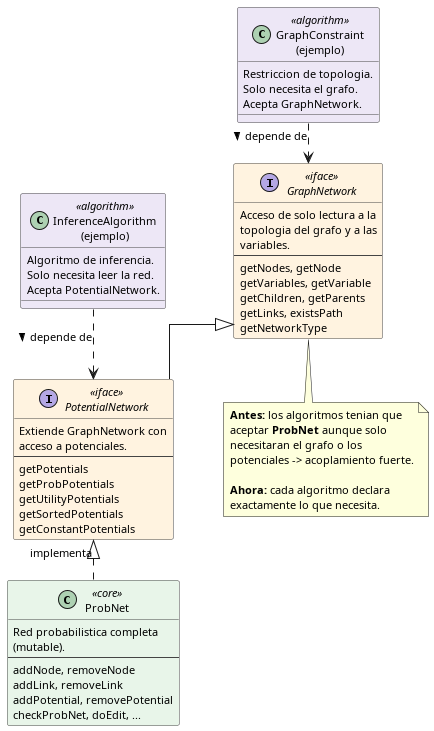
\includegraphics[width=0.85\textwidth]{interfaces.png}
  \caption{Jerarquía de interfaces.  Los algoritmos que solo necesitan el
           grafo dependen de \code{GraphNetwork}; los que necesitan
           potenciales, de \code{PotentialNetwork}.  \code{ProbNet} los
           implementa todos.}
  \label{fig:interfaces}
\end{figure}

\textbf{¿Por qué no se eliminó la API pública antigua?}  Algunos
métodos de \code{ProbNet} que antes se heredaban de \code{Graph} se
delegaban ahora explícitamente.  Esto hace visible que son operaciones
del grafo interno, no operaciones de dominio propias de la red.  Con el
tiempo, los llamadores pueden migrar a las interfaces.  Se añadió la
anotación \code{@Deprecated} a los métodos que ya no deberían usarse
directamente.

\textbf{Efecto en los algoritmos de restricción.}  Las restricciones de
red (\code{PNConstraint}) declaran ahora \code{checkProbNet(GraphNetwork
net)} en lugar de \code{checkProbNet(ProbNet net)}.  Esto redujo el
acoplamiento de las 35~clases de restricción, que ahora solo dependen de
la interfaz, no de la clase concreta.

\begin{lstlisting}[caption={Restricciones usando \texttt{GraphNetwork} en lugar de \texttt{ProbNet}.},
                   label=lst:constraint-iface]
// ANTES: cada restriccion dependia de la clase concreta ProbNet
public class NoCycleConstraint extends PNConstraint {
    @Override
    public boolean checkProbNet(ProbNet net, List<Variable> variables) {
        // ...usa net como ProbNet concreto...
    }
}

// DESPUES: la restriccion solo necesita la topologia del grafo
public class NoCycleConstraint extends PNConstraint {
    @Override
    public boolean checkProbNet(GraphNetwork net, List<Variable> variables) {
        // ...solo usa getNodes, getLinks, existsPath...
    }
}
\end{lstlisting}

% ===================================================================
\section{Resultado: arquitectura después del rediseño}
\label{sec:despues}

\subsection{Diagrama de la arquitectura actual}

La Figura~\ref{fig:after} muestra el diagrama UML de \code{ProbNet} y
sus clases satélite después del rediseño.

\begin{figure}[H]
  \centering
  
\includegraphics[width=\textwidth]{after.png}
  \caption{Arquitectura de \code{ProbNet} después del rediseño (1242~líneas).
           En \textcolor{pblue}{\textbf{azul}} se muestran las clases
           extraídas.  En naranja, las nuevas interfaces.}
  \label{fig:after}
\end{figure}

\subsection{Las clases extraídas}

\begin{center}
\begin{tabular}{lrp{7cm}}
\toprule
\textbf{Clase extraída} & \textbf{Líneas} & \textbf{Responsabilidad} \\
\midrule
\code{GraphNetwork}          &  92 & Interfaz: vista de solo lectura del grafo. \\
\code{PotentialNetwork}      &  47 & Interfaz: extiende \code{GraphNetwork} con potenciales. \\
\code{NetworkMetadata}       &  93 & Objeto valor: todos los metadatos descriptivos. \\
\code{ProbNetCopier}         & 168 & Copia superficial y profunda de la red. \\
\code{ProbNetClassifier}     &  90 & Consultas de clasificación (6 métodos estáticos). \\
\code{ProbNetAgentManager}   &  87 & Gestión de agentes (ADD/REMOVE/RENAME/UP/DOWN). \\
\code{ProbNetPotentialQueries} & 134 & Consultas complejas sobre potenciales. \\
\bottomrule
\end{tabular}
\end{center}

\subsection{Comparación de métricas}

\begin{center}
\begin{tabular}{lrrl}
\toprule
\textbf{Métrica} & \textbf{Antes} & \textbf{Después} & \textbf{Cambio} \\
\midrule
Líneas de \code{ProbNet.java}     & 1\,440 & 1\,242 & \good{$-$14\%} \\
Campos en \code{ProbNet}          & 16     & 7      & \good{$-$56\%} \\
Bugs conocidos                    & 4      & 1*     & \good{$-$75\%} \\
Code smells                       & 7      & 0      & \good{$-$100\%} \\
Clases en el paquete \code{network} & ---  & +7     & (nuevas clases satélite) \\
Restricciones acopladas a \code{ProbNet} & 35 & 0  & \good{todas usan \code{GraphNetwork}} \\
\bottomrule
\end{tabular}
\end{center}

{\small * Bug B4 (\code{addShiftedNode()} sin potenciales) permanece documentado
con \code{@ToCheck} hasta que se decida el comportamiento correcto.}

\subsection{Qué no cambió}

La API pública de \code{ProbNet} no se rompió en ningún punto: todos los
métodos que existían antes siguen existiendo con la misma firma.  Los
490~ficheros que referencian a \code{ProbNet} no necesitaron
modificación alguna para que los tests pasaran.  Esto fue posible gracias
a las delegaciones que \code{ProbNet} conserva hacia las clases extraídas.

La migración progresiva está disponible: los llamadores pueden ir
adoptando las nuevas clases de utilidad (\code{ProbNetClassifier.isMultiagent(net)}
en lugar de \code{net.isMultiagent()}) o las interfaces
(\code{GraphNetwork} en lugar de \code{ProbNet}) cuando sea conveniente,
sin ninguna urgencia.

% ===================================================================
\section{Orden de ejecución y riesgos}

Las fases se ejecutaron con el siguiente orden y nivel de riesgo:

\begin{center}
\begin{tabular}{clcl}
\toprule
\textbf{Fase} & \textbf{Descripción} & \textbf{Riesgo} & \textbf{Estado} \\
\midrule
1 & Corrección de bugs B1--B3 y smells S1--S7   & Bajo   & \good{Completada} \\
  & Extracción de \code{NetworkMetadata}         & Bajo   & \good{Completada} \\
  & Extracción de \code{ProbNetCopier}           & Bajo   & \good{Completada} \\
3 & Extracción de \code{ProbNetClassifier}       & Medio  & \good{Completada} \\
4 & Extracción de \code{ProbNetAgentManager}     & Bajo   & \good{Completada} \\
5 & Extracción de \code{ProbNetPotentialQueries} & Medio  & \good{Completada} \\
  & Introducción de \code{GraphNetwork}/\code{PotentialNetwork} & Alto & \good{Completada} \\
  & Adaptar restricciones a \code{GraphNetwork}  & Medio  & \good{Completada} \\
--& Resolución de bug B4 (\code{addShiftedNode}) & Bajo   & \warn{Pendiente} \\
--& Mover \code{reader}/\code{writer} a la GUI   & Alto   & \warn{Pendiente} \\
\bottomrule
\end{tabular}
\end{center}

Las dos tareas pendientes son independientes del resto del rediseño.
La primera requiere consultar el comportamiento esperado en la GUI.
La segunda requiere un análisis de impacto en los módulos \code{gui} e
\code{io}.

% ===================================================================
\begin{thebibliography}{9}

\bibitem{fowler2019}
  M.~Fowler,
  \emph{Refactoring: Improving the Design of Existing Code},
  2nd ed., Addison-Wesley, 2019.

\bibitem{martin2003}
  R.~C.~Martin,
  \emph{Agile Software Development: Principles, Patterns, and Practices},
  Prentice Hall, 2003.

\bibitem{gamma1995}
  E.~Gamma, R.~Helm, R.~Johnson, J.~Vlissides,
  \emph{Design Patterns: Elements of Reusable Object-Oriented Software},
  Addison-Wesley, 1995.

\bibitem{hunt1999}
  A.~Hunt, D.~Thomas,
  \emph{The Pragmatic Programmer},
  Addison-Wesley, 1999.

\end{thebibliography}

\end{document}
